\singlespacing
\begin{figure}[H]
    \centering
    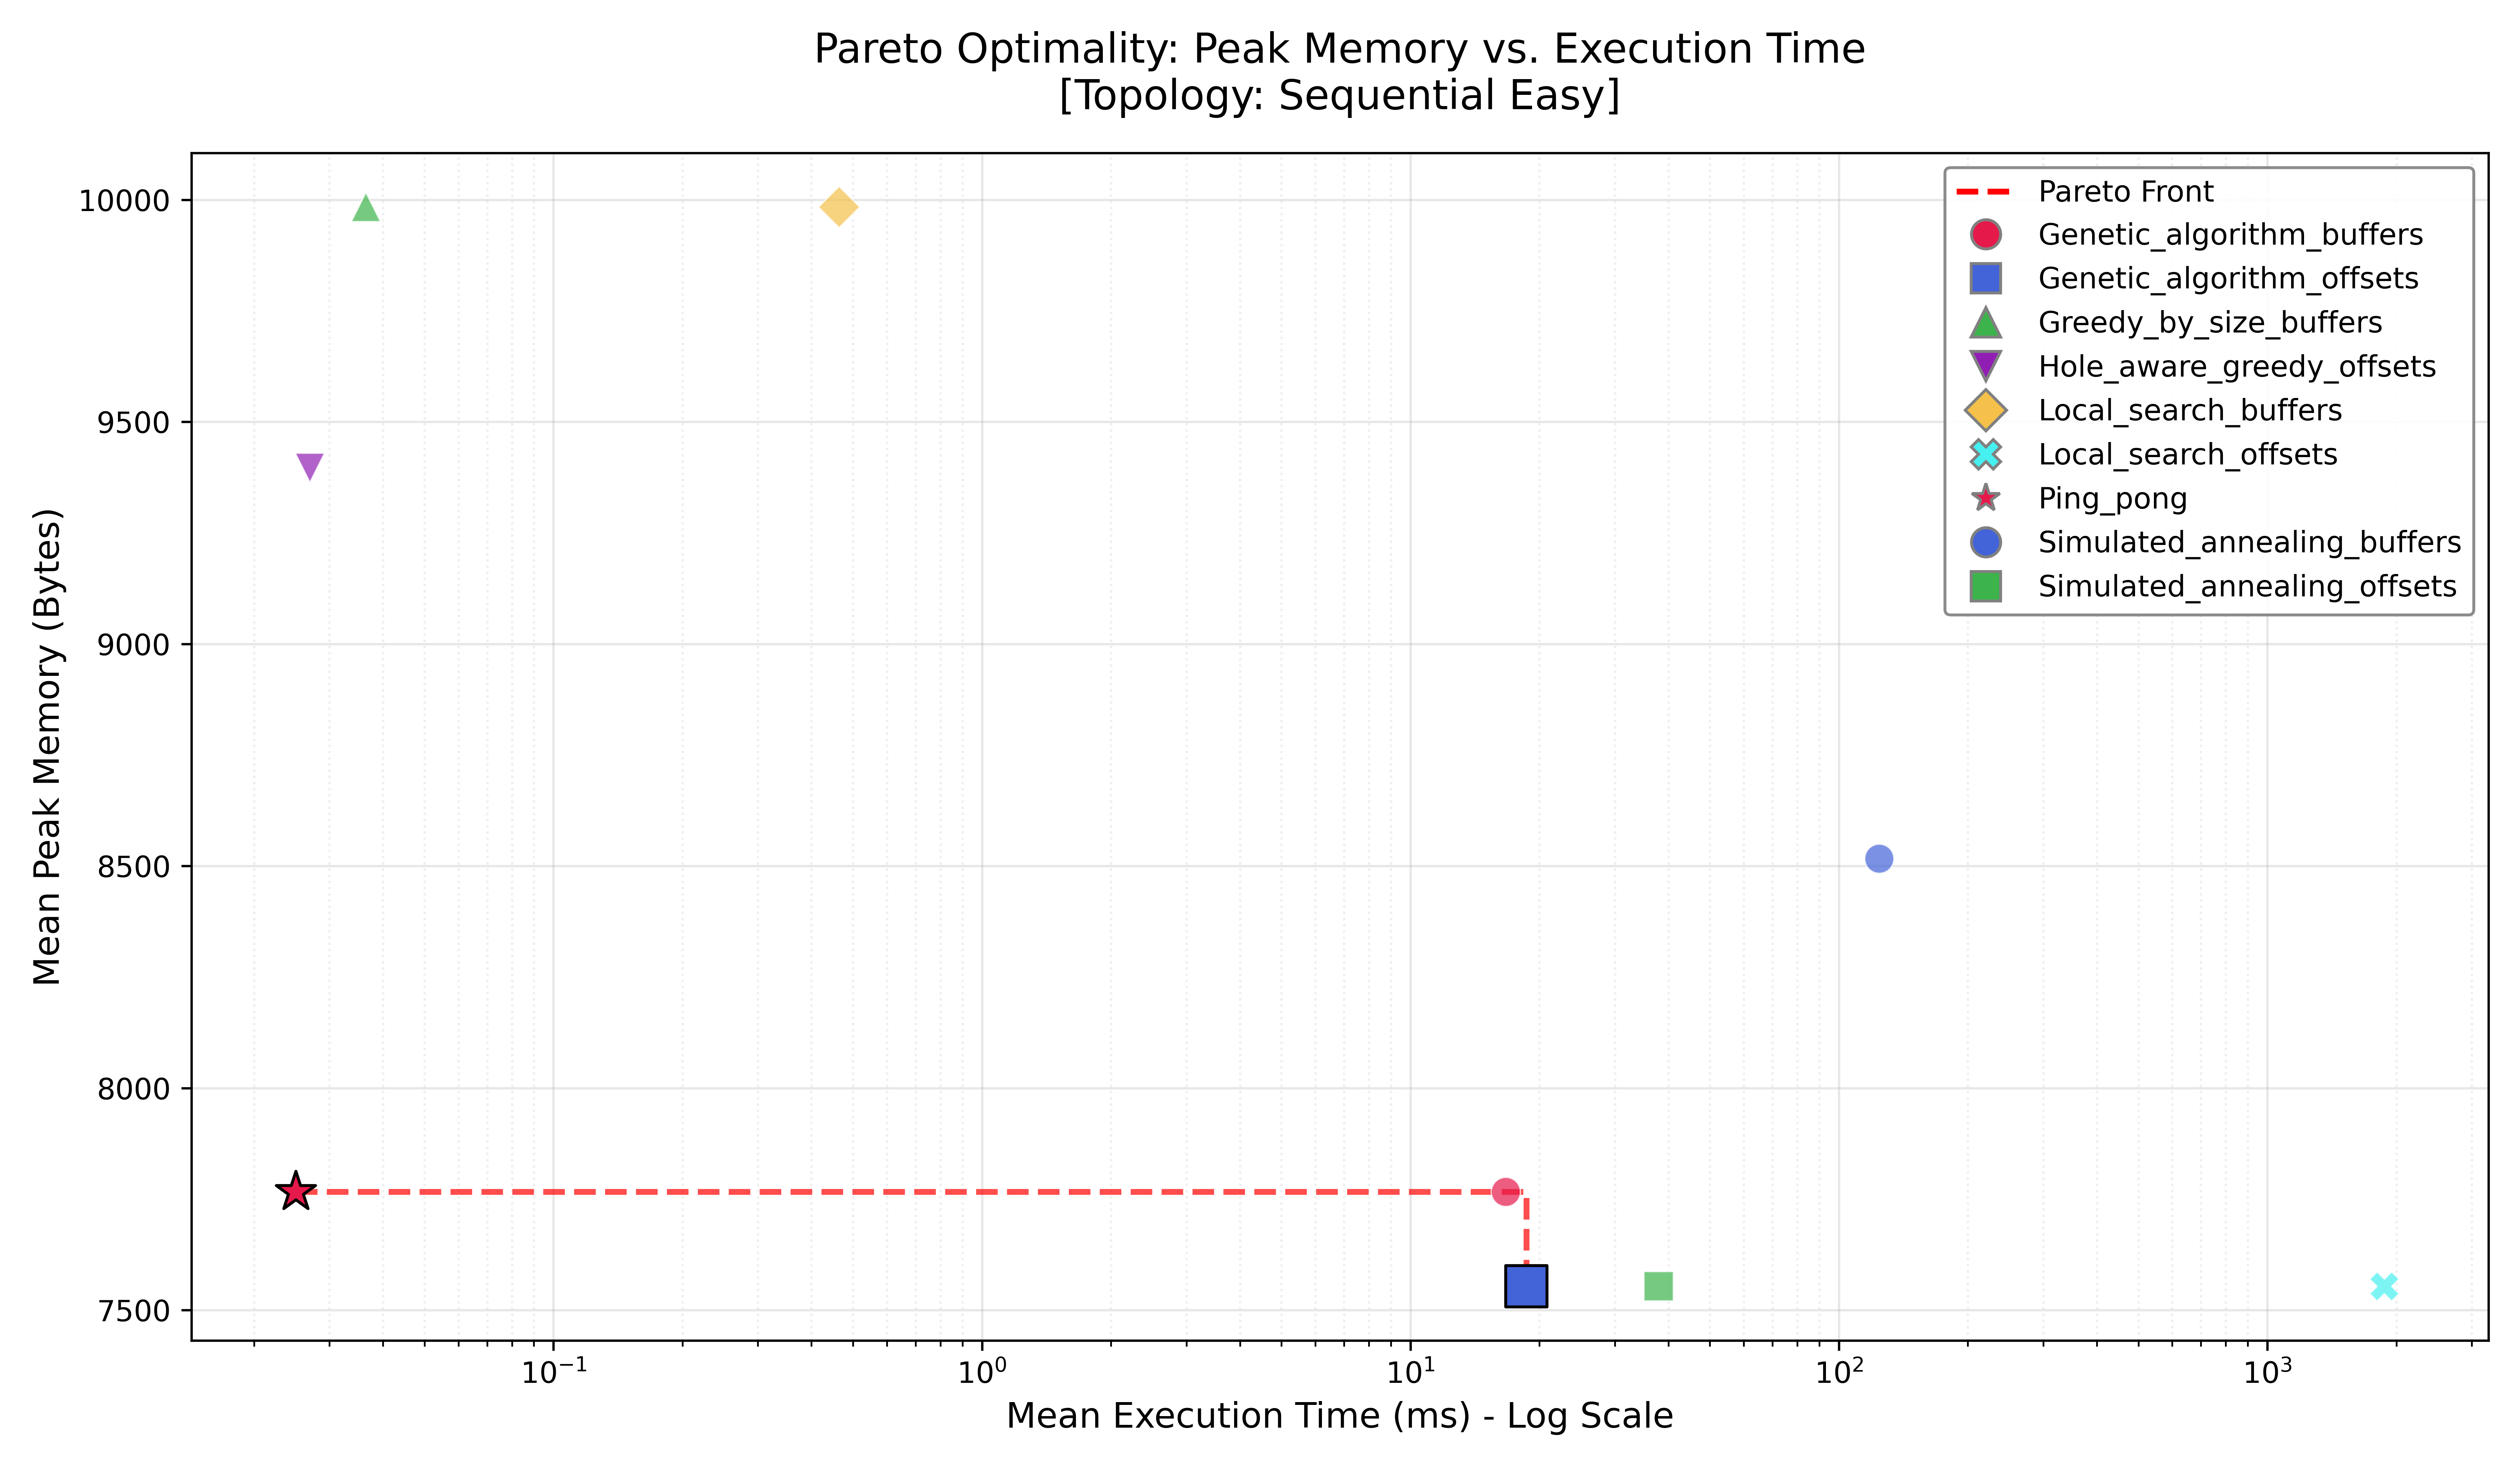
\includegraphics[width = 1\textwidth ]{figures/pareto_sequential.png}
    \caption{Memory allocation of Hole-aware Greedy algorithm in forkjoin networks}
    \label{Figure6}
\end{figure}
Figure 6 illustrates the Pareto front with respect to mean execution time and mean maximum memory consumption under 10 different Sequential topologies. The Ping-pong algorithm emerges as the most efficient way, occupying the ideal bottom-left region with sub-millisecond latency (0.025 ms) and a competitive memory footprint. Furthermore, Genetic Algorithm based on offsets achieves the minimum peak memory consumption across all tested candidates. However, as a meta-heuristic approach, it necessitates a longer runtime to converge compared to the more direct Ping-pong strategy.

\begin{figure}[H]
    \centering
    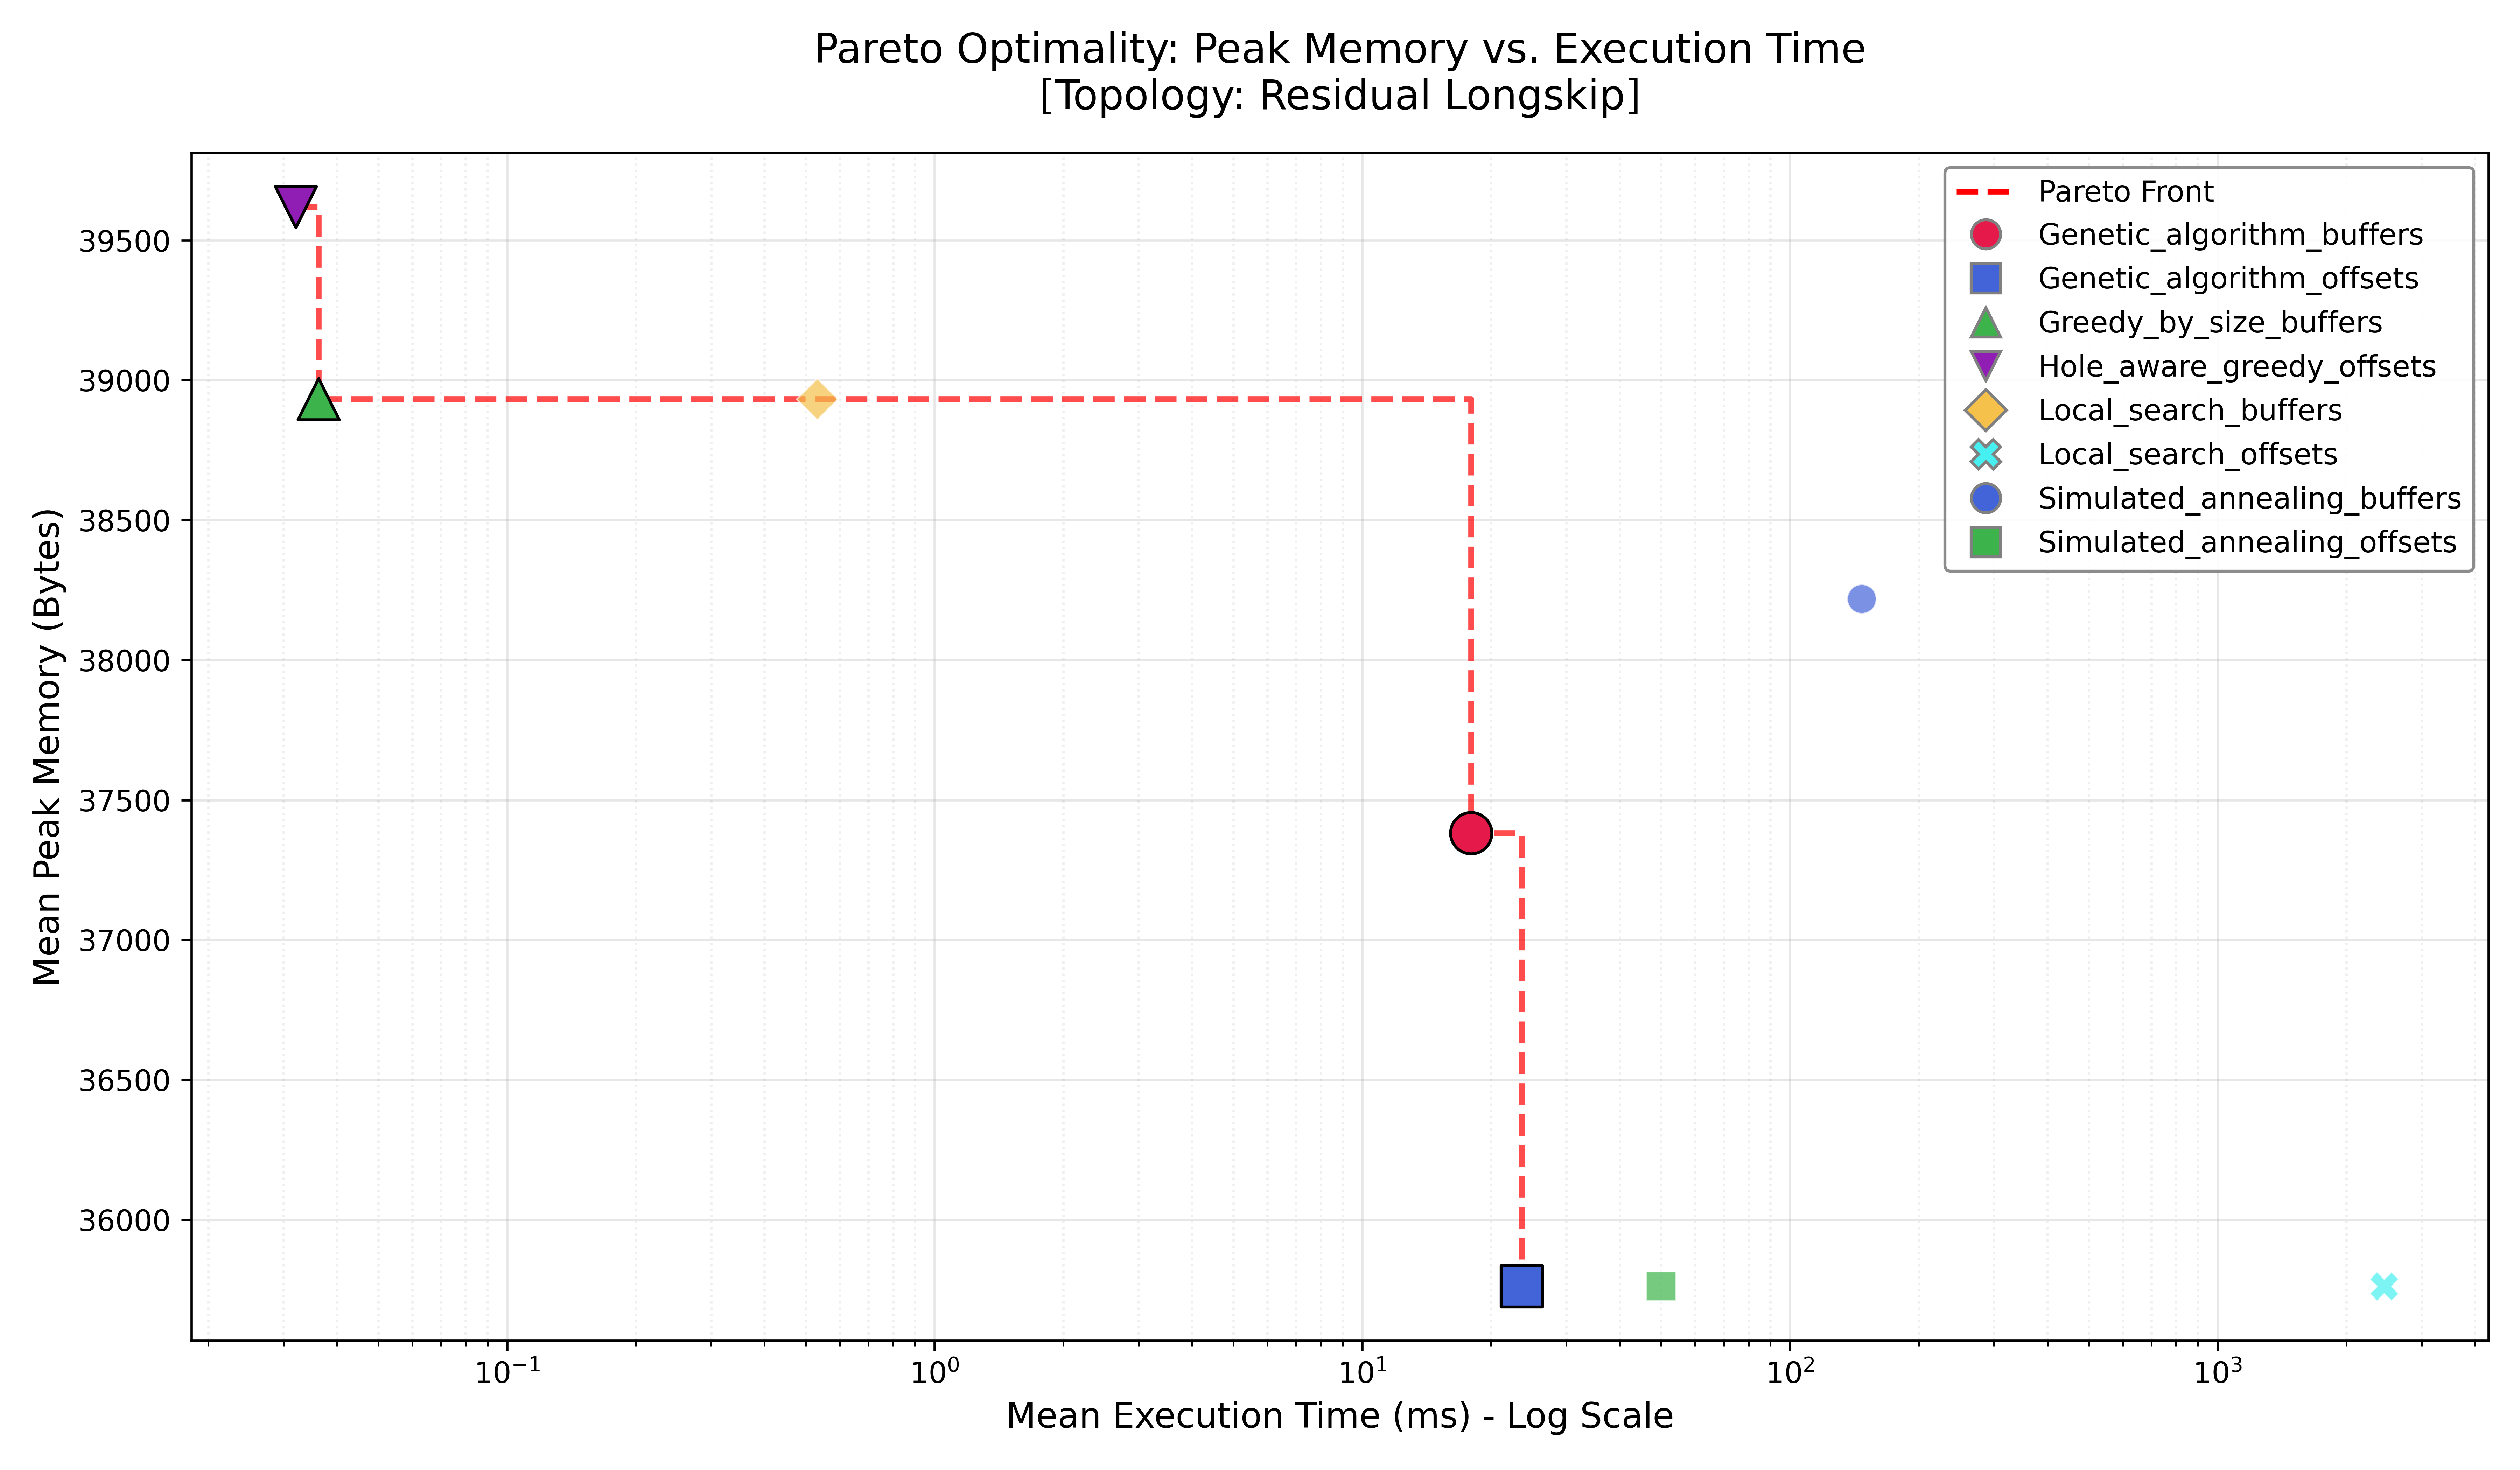
\includegraphics[width = 1\textwidth ]{figures/pareto_residual.png}
    \caption{Memory allocation of Hole-aware Greedy algorithm in forkjoin networks}
    \label{Figure7}
\end{figure}
\begin{figure}[H]
    \centering
    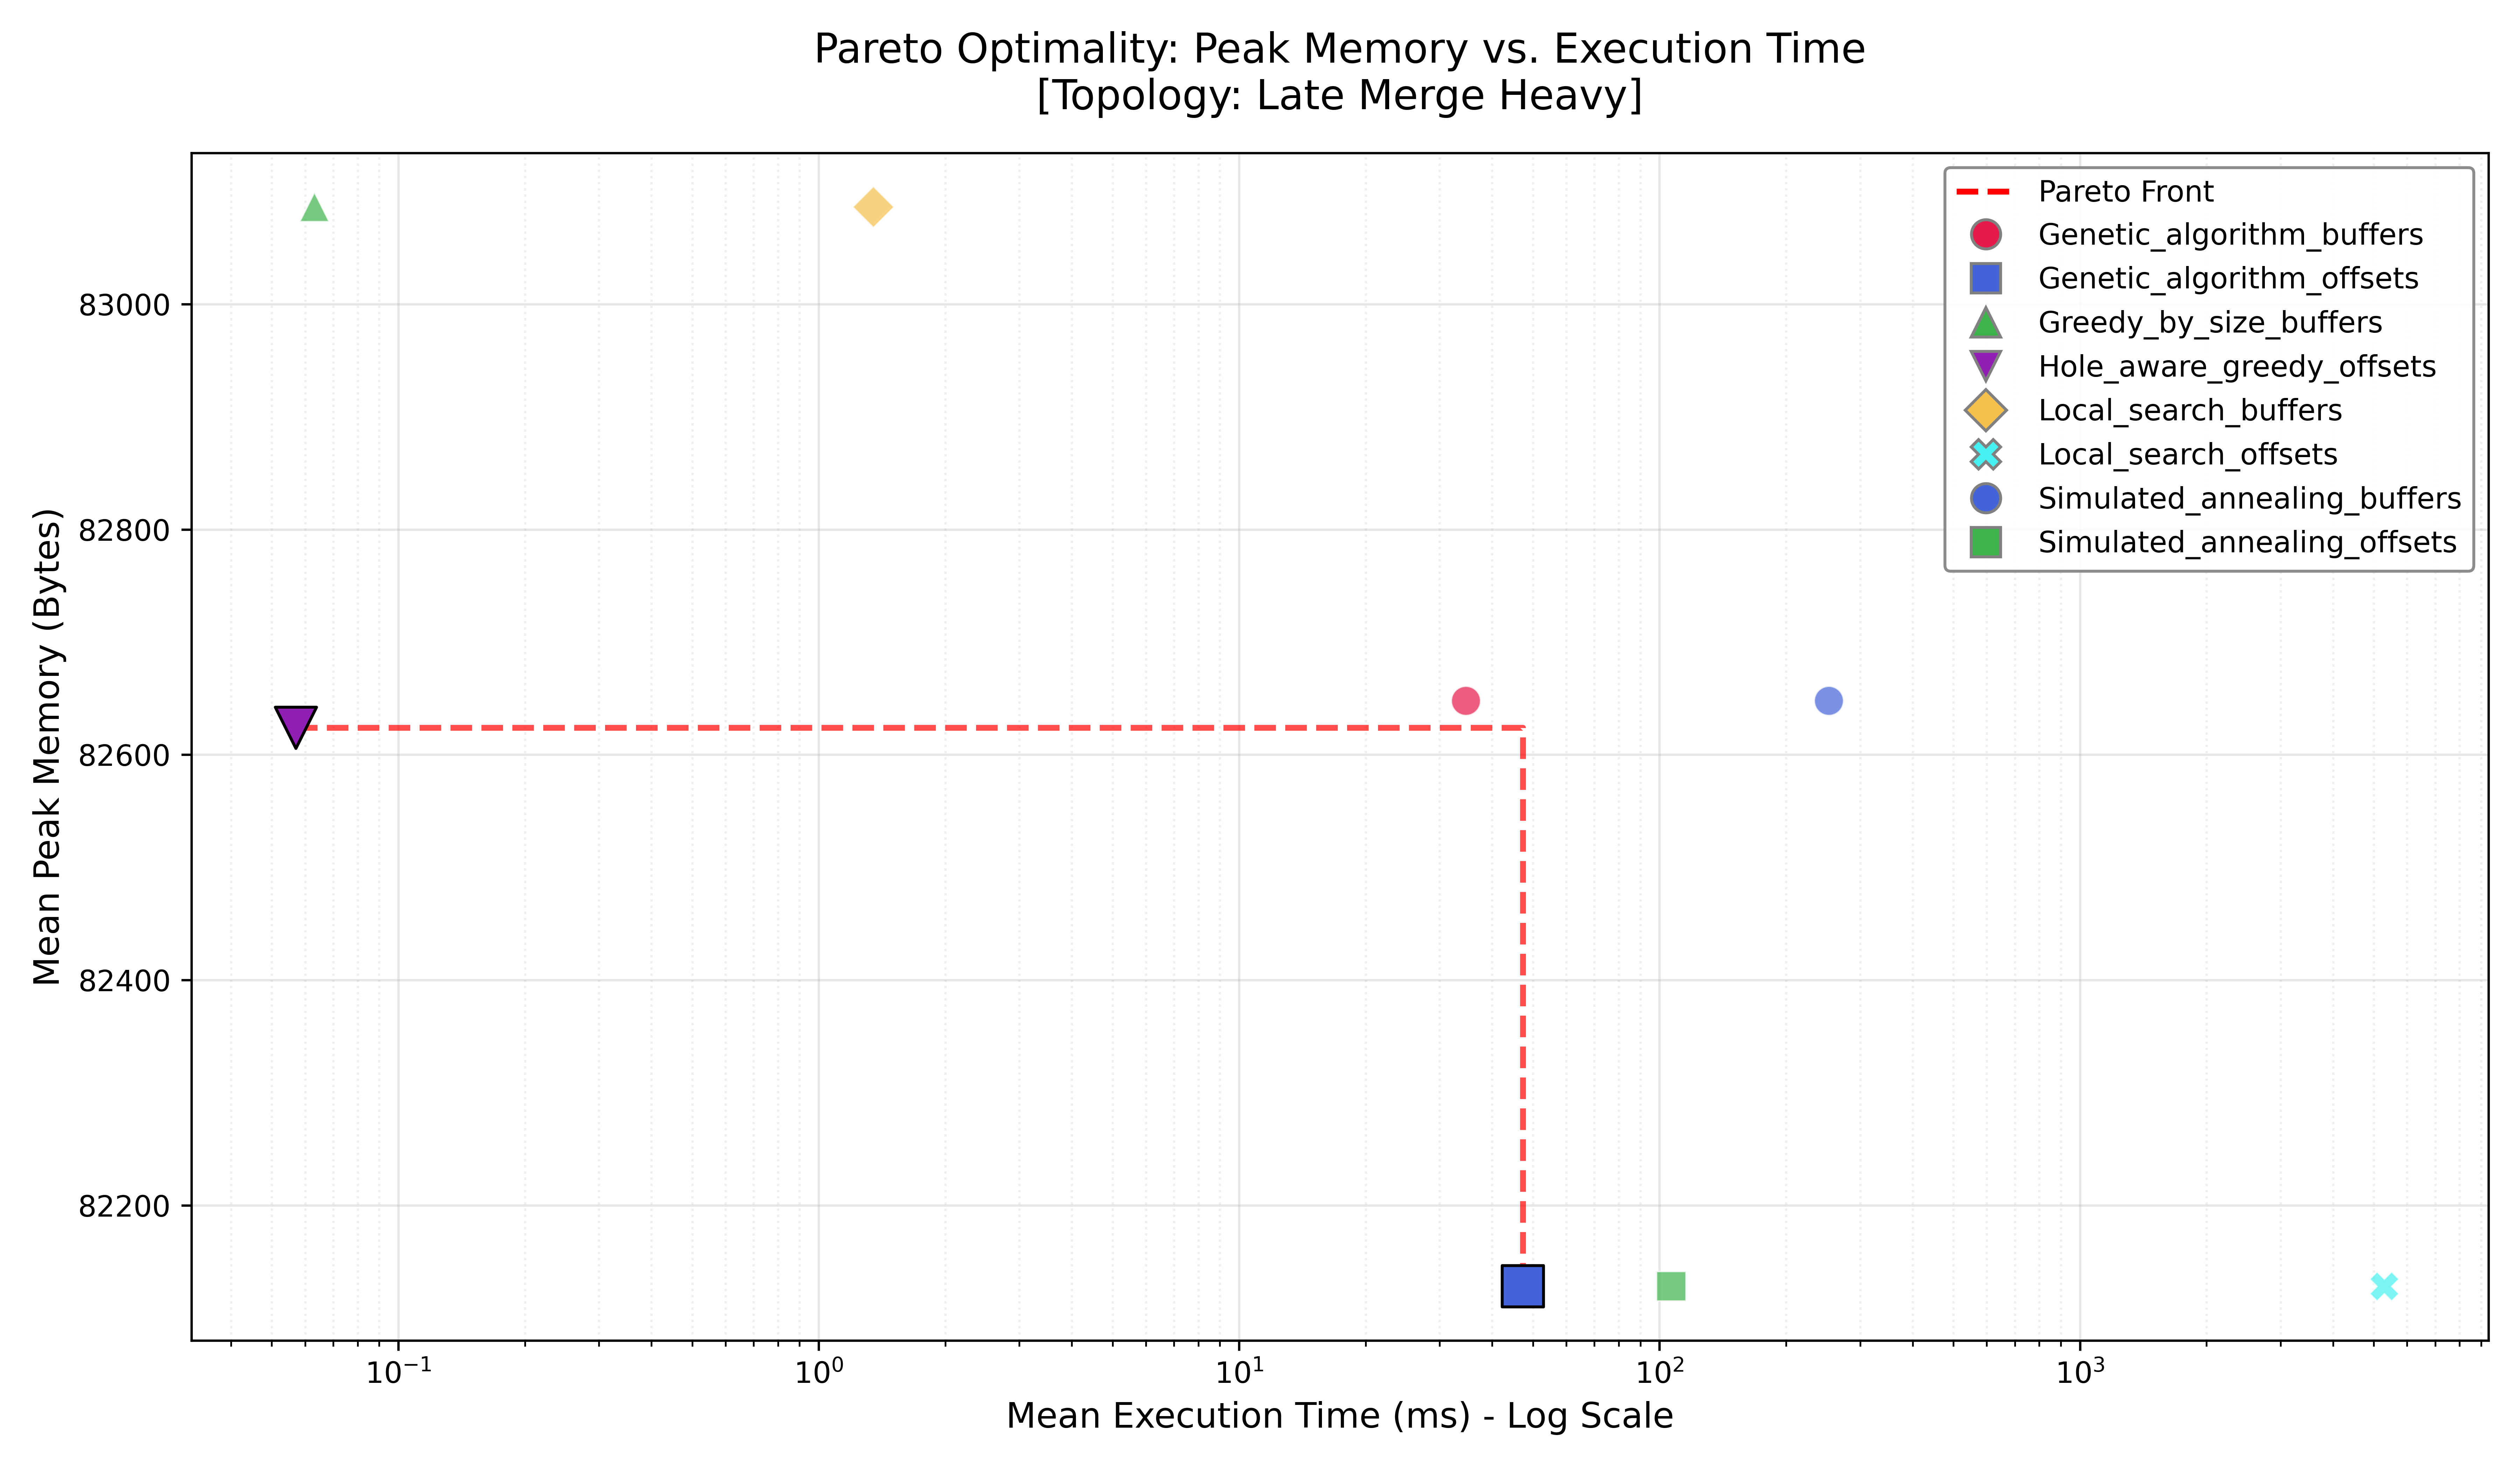
\includegraphics[width = 1\textwidth ]{figures/pareto_late_merge.png}
    \caption{Memory allocation of Hole-aware Greedy algorithm in forkjoin networks}
    \label{Figure8}
\end{figure}
\begin{figure}[H]
    \centering
    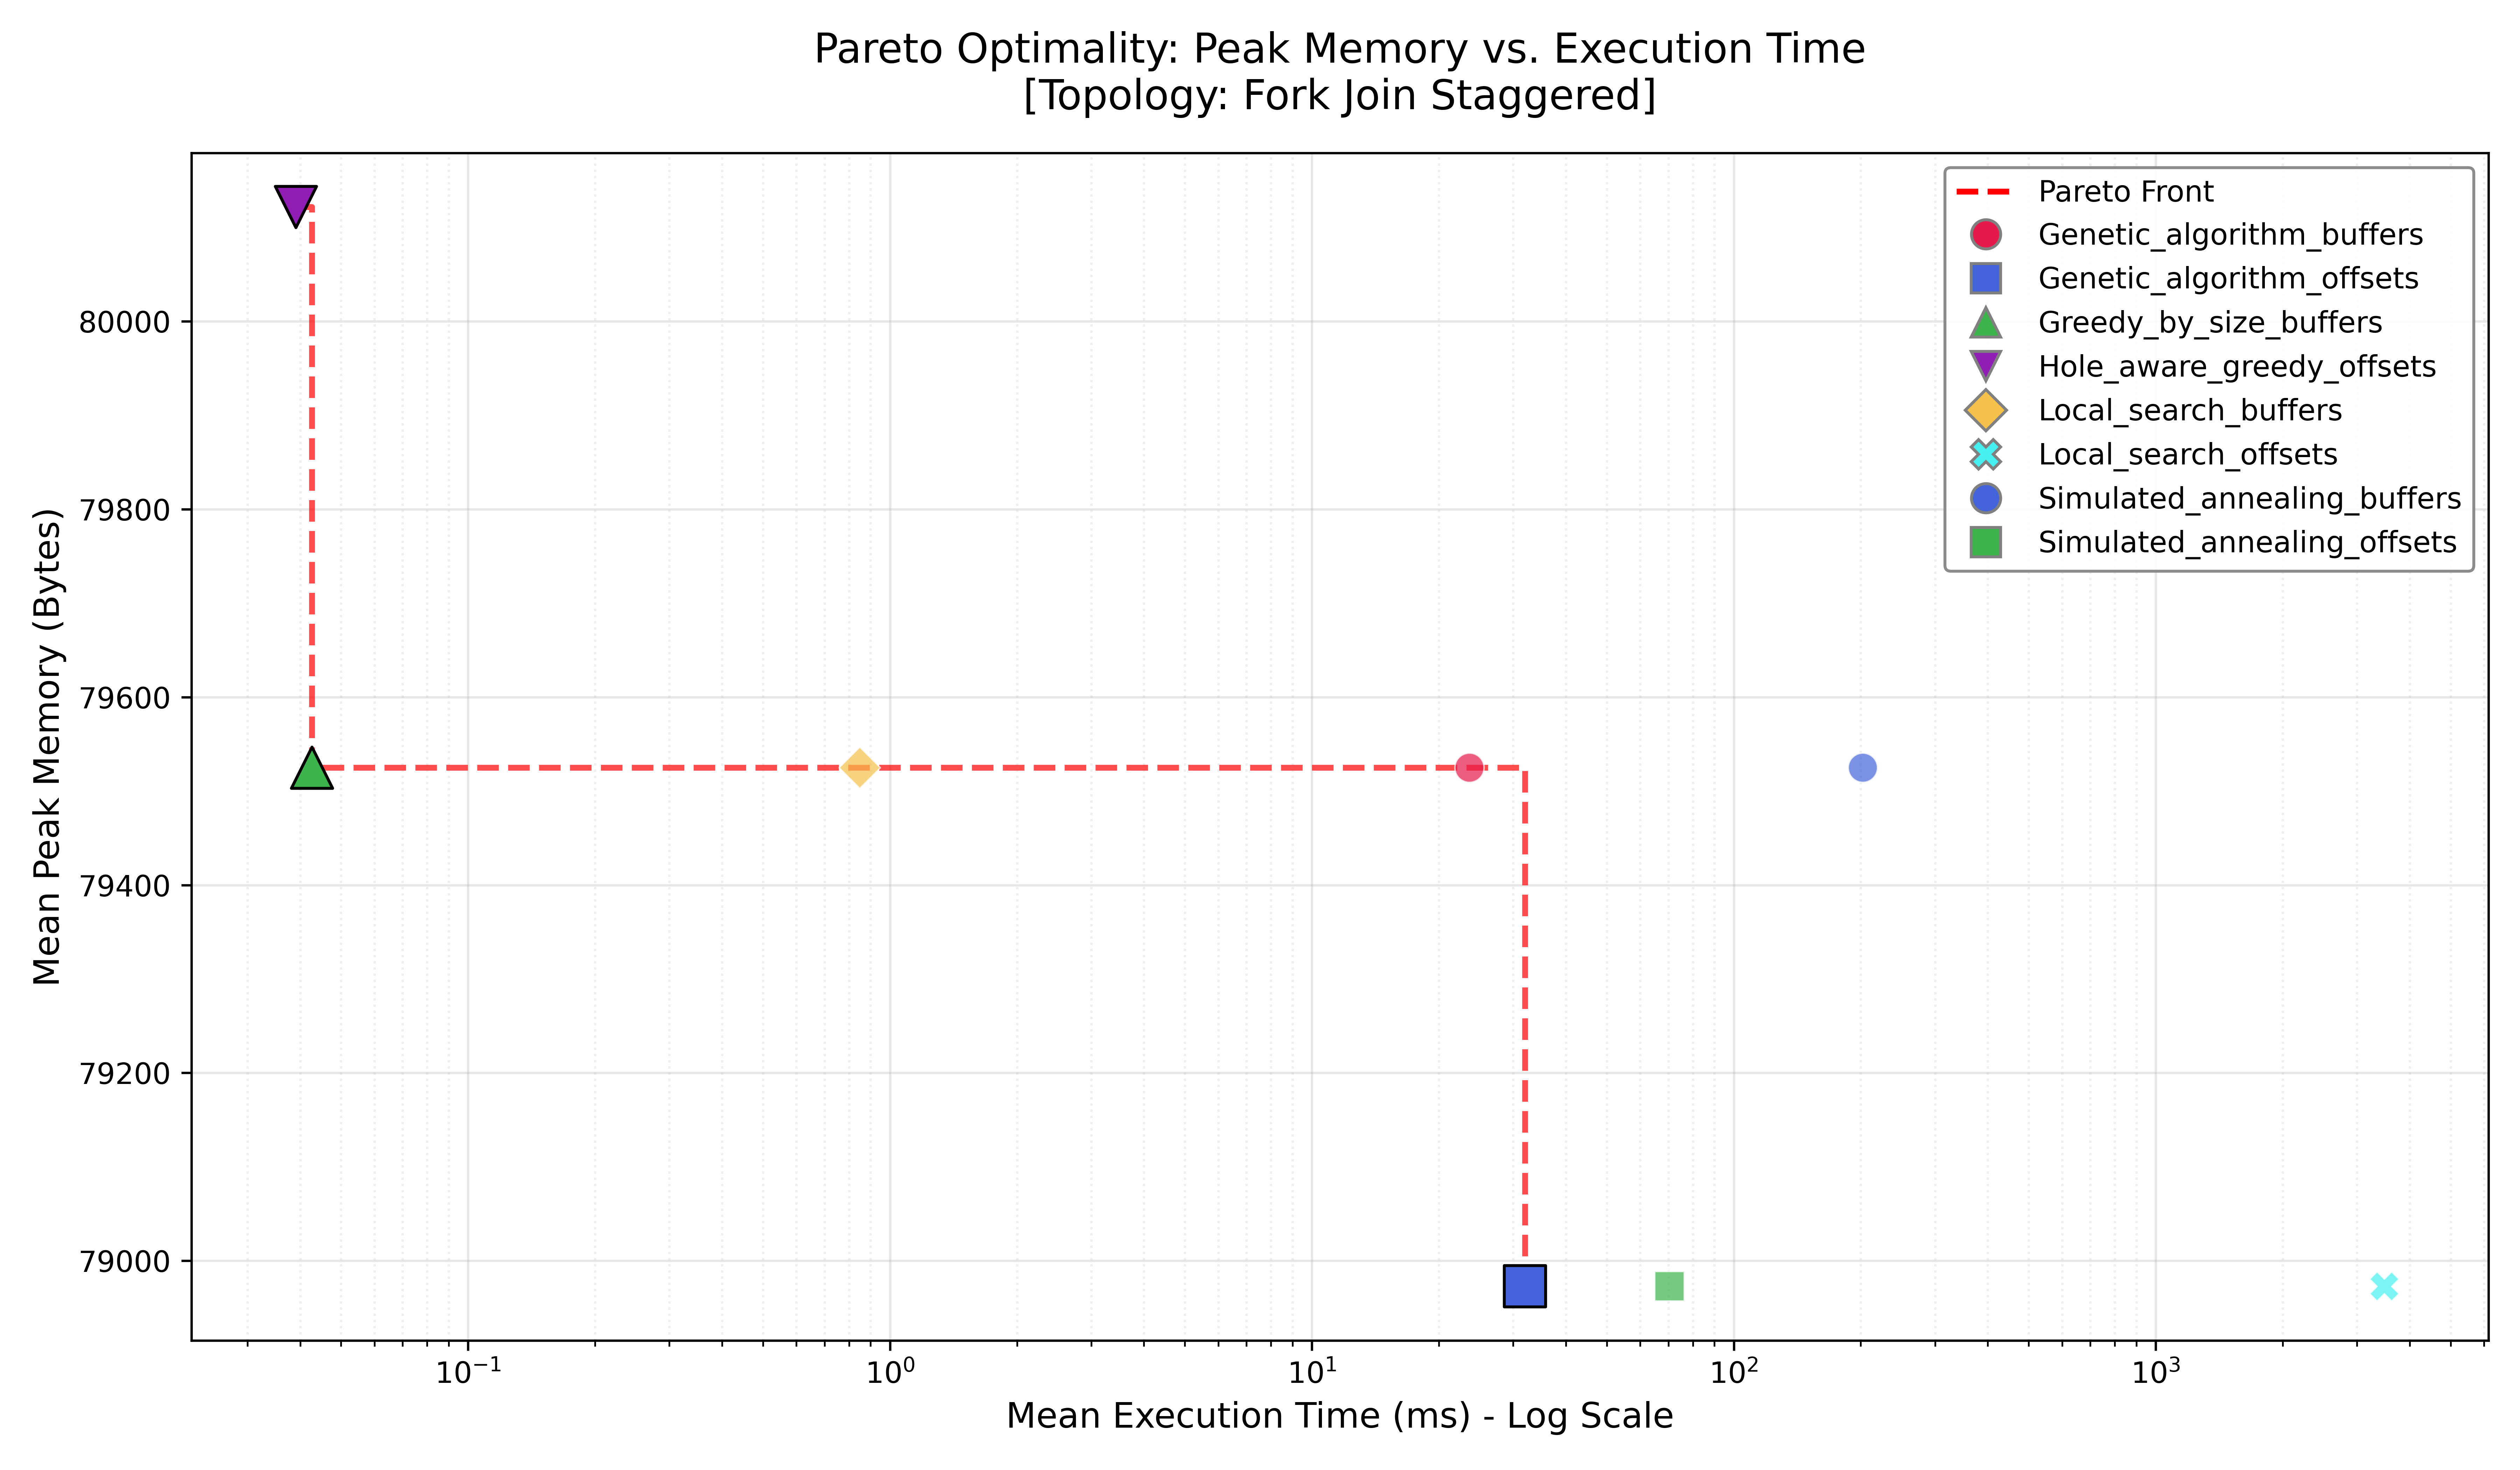
\includegraphics[width = 1\textwidth ]{figures/pareto_fork_join.png}
    \caption{Memory allocation of Hole-aware Greedy algorithm in forkjoin networks}
    \label{Figure9}
\end{figure}
In other three examined topologies-Fork Join, Late Merge, and Residual networks,as shown in Figure 7, 8 and 9, a consistent trend is observed. The Hole-aware Greedy algorithm offers the fastest execution speed. In most cases, it successfully identifies memory layouts with a lower peak memory than standard Greedy by Size algorithms, although its superiority is not absolute across all complex topologies.

Among the evaluated meta-heuristic algorithms, the Genetic Algorithm dominates others' performance, achieving the most effective optimization with the highest computational efficiency. In contrast, Local Search and Simulated Annealing exhibit a tendency to become trapped in local optima; even in scenarios where they eventually reach a solution comparable to that of the GA, they consume significantly longer convergence times.

Overall, the results confirm that while the structural complexity of the computation graph dictates the baseline memory requirement, the GA-based meta-heuristic combined with an offset-based allocation represents the most robust approach for reaching the theoretical limit of resource efficiency. In the Fork Join Staggered topology, Greedy by Size emerges as a viable candidate for balancing peak memory and computational overhead. Similarly, in Residual structures, both Greedy by Size and Genetic Algorithm based on buffers provide competitive trade-offs.
